% chktex-file 8

\chapterimage{penguin.jpg} 
\chapter{Piazza}\label{C:piazza}

\FILENAME\

We use Piazza (\url{https://piazza.com}) because questions and answers
on Piazza are community-edited and provides the opportunity not only
for instructors, but also for students to contribute. Each question
has a single answer edited by the students of the class and if needed
an instructors' answer that is collaboratively edited by the
instructors.

Due to this wiki-style Q\&A, when a student has a question, one does not
have to look through long e-mail threads but instead can look at the
answer. For details that lead up to the answer you are highly encouraged
to also look at some comments that lead up to the answer.

An advertisement video from Piazza summarizes the features:

  \URL{https://www.youtube.com/watch?v=2jLSiN8E18w}

Piazza Support with a lot of information is available at:

  \URL{http://support.piazza.com}

A good document about piazza is available at

  \URL{https://piazza.com/pdfs/piazza_product_introduction.pdf}

\section{Access to Piazza from Canvas}

Piazza is one of the recommended IU supported technologies within
CANVAS. It replaces the CANVAS discussion groups with superior
technology targeted to support large student classes while also
focussing on student engagement.

To access piazza you can have the following situations provided in the
next four subsections. Please read \emph{ALL}* of them
\textbf{CAREFULLY}, decide which applies tou you and follow the
instructions. If you have improvements to this instructions, please let
us know.

\subsection*{Situation: You have never logged into piazza}

First, Click the Piazza link on the left navigation of your Canvas
course.

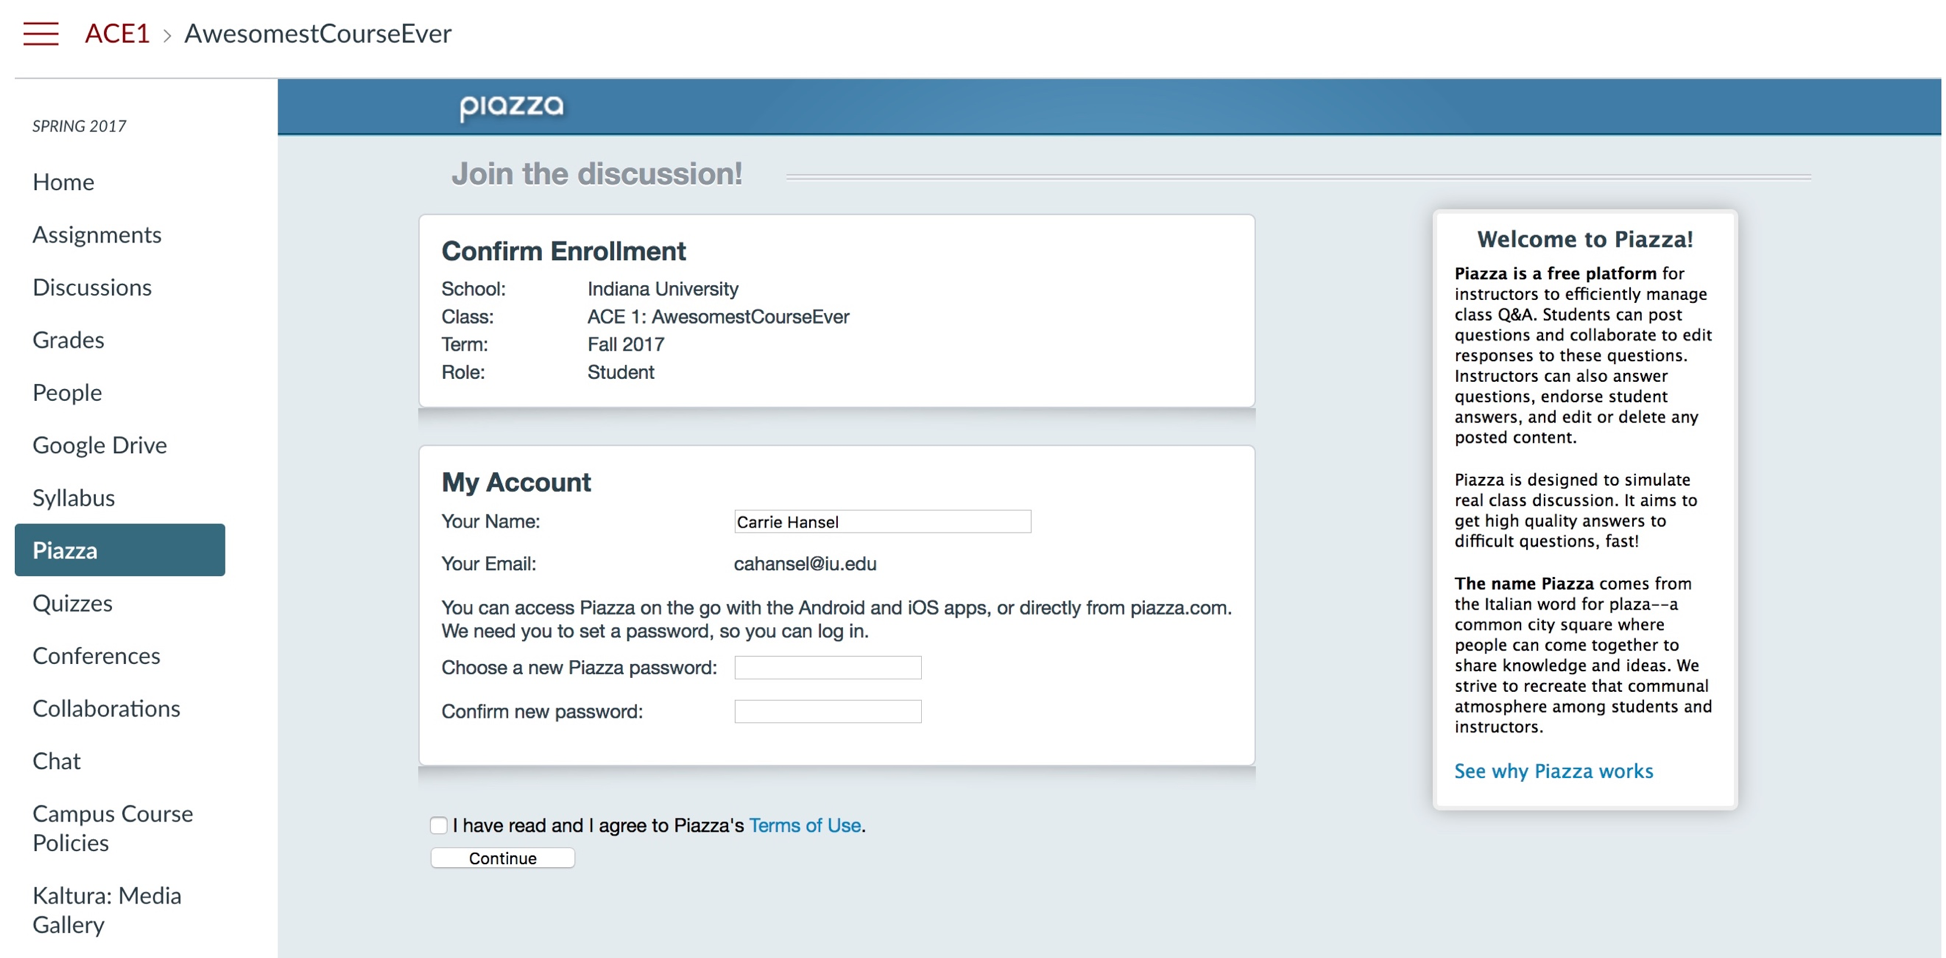
\includegraphics[width=0.75\textwidth]{images/piazza/image3.png}

Second, create password and accept terms.


The email address shown on this screen is your default IU
email address. It is the address Canvas sends to all integrated tools
like Piazza. You can not edit it, so do not try.

The password you create here is for accessing Piazza from a
mobile device. You must~use the default IU email address from this
screen to access this account on another device, so make a note of it.

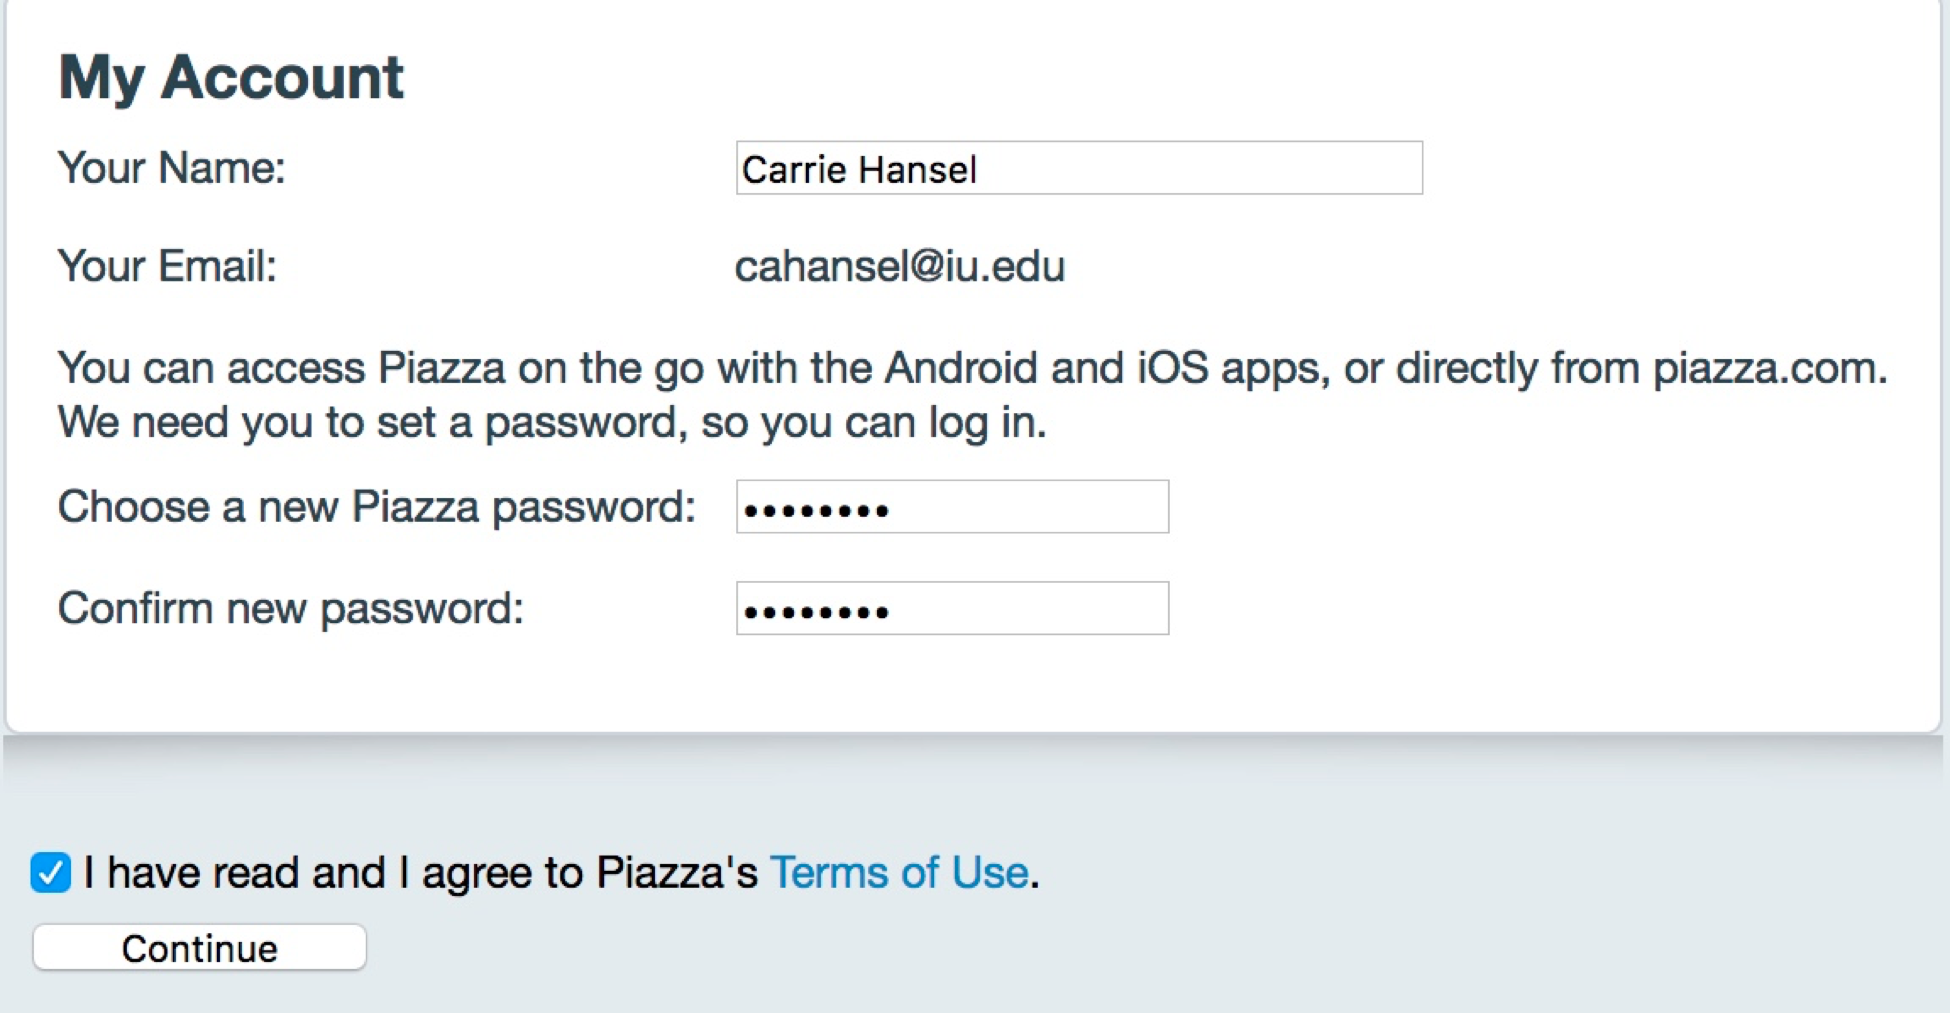
\includegraphics[width=0.75\textwidth]{images/piazza/image1.png}

Choose current degree program (only important if you want to opt into
their recruiting program on the next screen; choose whatever you want
here)

Third, associate your IU account

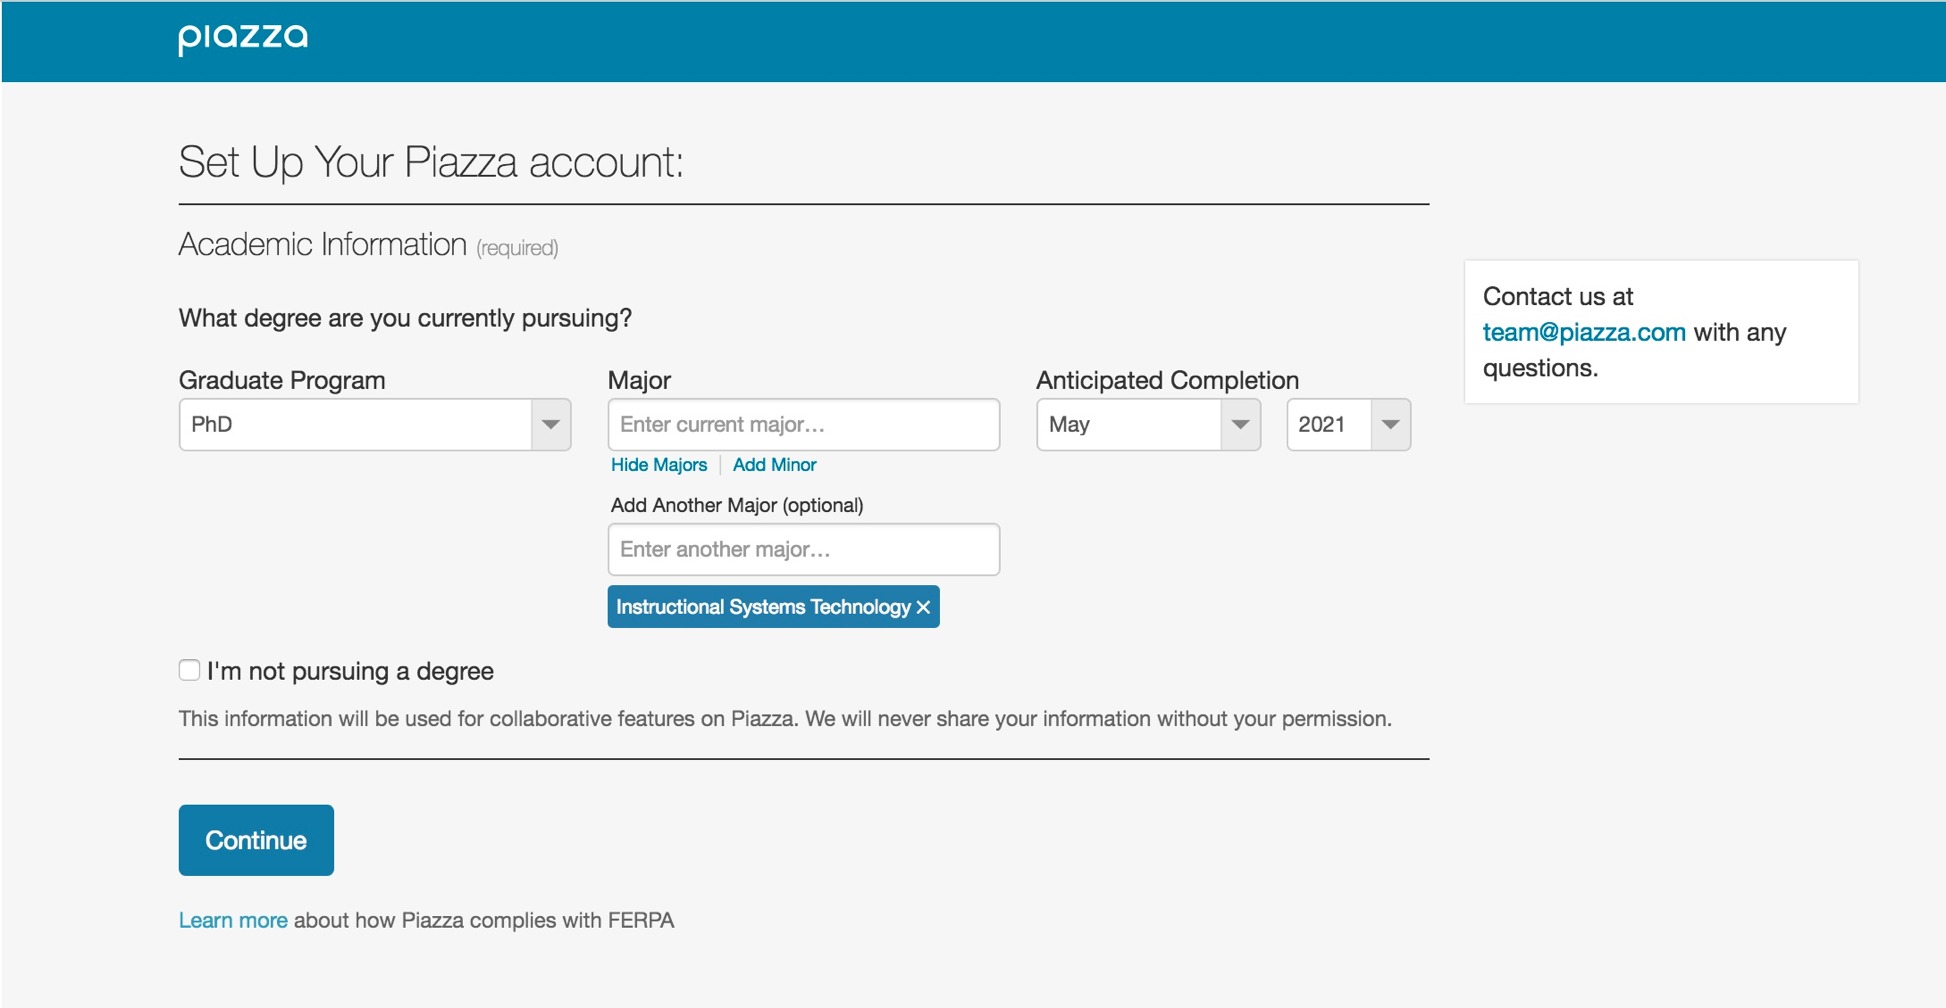
\includegraphics[width=0.75\textwidth]{images/piazza/image4.png}

Forth, if all goes well you see the Success screen

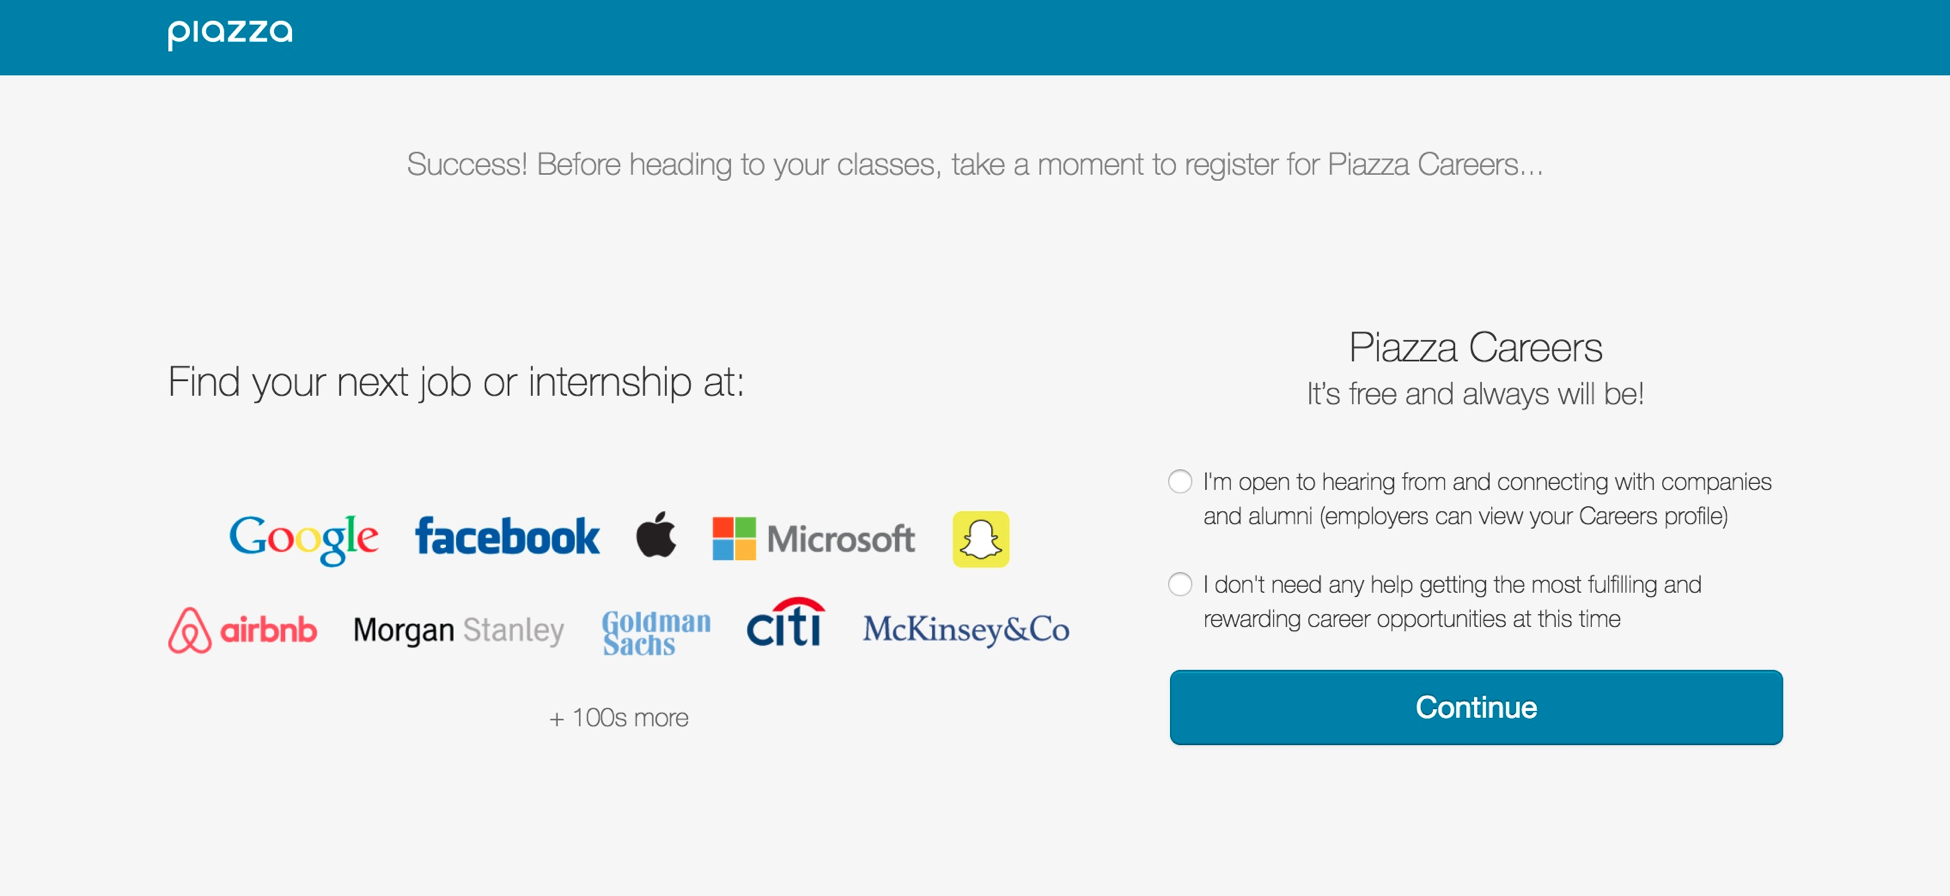
\includegraphics[width=0.75\textwidth]{images/piazza/image2.png}

\subsection*{Situation: You have logged into piazza and used your
  default IU e-mail}

\begin{enumerate}
\item Click the Piazza link on the left navigation of your Canvas
  course.
\item You will be automatically enrolled in the course Piazza site and
  logged in.
\item Start using Piazza.
\end{enumerate}

\subsection*{Situation: You have logged into piazza and you used
another non IU
e-mail}\label{situation-you-have-logged-into-piazza-and-you-used-another-non-iu-e-mail}

\begin{enumerate}
\item
  Click the Piazza link on the left navigation of your Canvas course.
\item
  Proceed as in \#1 above. This will create your new Piazza account that
  is linked to your courses in Canvas. This is the account you should
  always use in your IU courses.
\item
  If you wish to merge other accounts that you own, please see
  \href{https://www.google.com/url?q=http://support.piazza.com/customer/portal/articles/1646661-add-an-email-address-or-merge-two-accounts\&sa=D\&ust=1502127148503000\&usg=AFQjCNHyBFh3TMAtSDpFordYOfH0IE6kPA}{Add
  an email address or merge two accounts}.
\end{enumerate}

\subsection*{Situation: You have multiple accounts in piazza}

\begin{enumerate}

\item
  If one of your multiple accounts corresponds with your default IU
  email address, you will be automatically enrolled in the course Piazza
  site and logged in.
\item
  If none of your accounts corresponds to your default IU email address,
  follow the instructions in \#3 above.
\item
  If you wish to merge other accounts that you own, please see
  \href{https://www.google.com/url?q=http://support.piazza.com/customer/portal/articles/1646661-add-an-email-address-or-merge-two-accounts\&sa=D\&ust=1502127148504000\&usg=AFQjCNHwO1kks2cnVLpWWCnOIEDFhl2fJA}{Add
  an email address or merge two accounts}.
\end{enumerate}

I post the official response form the CANVAS team here:
``When a student clicks the Piazza link in your course navigation, they
will be authenticated through to Piazza. If the student already has a
Piazza account that matches their default Canvas email, they will simply
be enrolled in the Piazza course. If the student doesn't have an
account, Canvas sends the pertinent information (default email address
primarily) to Piazza, Piazza creates the student's account and enrolls
the student in the Piazza course. There is nothing you need to do to.''

If you have any questions regarding accessing piazza, please send them
to

``Ricci, Margaret P''
\textless{}\href{mailto:mricci@iu.edu}{\nolinkurl{mricci@iu.edu}}\textgreater{}

\section{Verify you are on Piazza via a post}

Post on the \textbf{bio} folder a short introduction about yourself. One
that you could include in a paper.

An example is provided at \url{https://laszewski.github.io/bio.html}
with an image at \url{https://laszewski.github.io/_images/gregor.jpg}

Use the subject line \emph{Biography: Firstname Lastname} and post it
into the bio folder.

\section{Making Piazza Work}

In order for Piazza to work students and instructors need to participate

\textbf{Students participate:} Students must collaboratively work on an
answer to a question. Students must not post irrelevant followups to a
question. If you notice your comment was irrelevant, please delete it.
Students must \textbf{search} prior to asking a new question if the
question has already been asked. Duplicated questions can be merged.

\textbf{Instructors guide:} The instructor guides the students in order
to obtain an answer to a question. In some cases the instructor may be
the only one knowing the answer in which case he tries to provide it.

\textbf{Not using e-mail:} Instructors will and must not use e-mail to
communicate with a student. All communication will be done via piazza.
There, are only very view situations where e-mail is allowed, ask on
piazza first if you should engage in e-mail conversations.

\textbf{Not using CANVAS discussions:} We will not engage in any CANVAS
message exchange. Any communication is to be done on Piazza. It is in
your responsibility to enroll in Piazza to make it work for you.
Instructions are posted in this document. (Grade discussion will be
done in CANVAS)

\section{Towards good questions}

Naturally when you ask a question you need to do it in a reasonable form
and provide sufficient information so that the question can be answered.
It is in the responsibility of the student to update the question to
provide enough information.

Thus information may include: Firstname Lastname, HID, and URL
to document in question

To give you an example of a \textbf{bad} question consider:

\begin{verbatim}
*send from Xi Lee*

Hi Professor:

I read a nice article about apples and potato's and updated my
paper. Please give me feedback

Thank you

Kevin
\end{verbatim}

Here the reasons why this can be improved:

\begin{enumerate}
\item
  As professors and instructors may review your document it is
  unnecessary to start with ``Hi Professor:'', just leave it away. If
  you want a particular instructor use the name explicitly, such as
  ``Gregor:'', e.g.\ multiple professors may be teaching your course.
\item
  You have not specified which article you read, you need to include the
  URL to the article so we can follow your argument.
\item
  You have not included the link to your document so we do not know what
  you are talking about. Remember there are many others students in the
  class
\item
  You are using a different name from the one that you are registered
  with. This can lead to confusion when we look up your name. We prefer
  that you use only one name that is associated with your e-mail.
\end{enumerate}

The above question will simply be commented on (if at all):

``Missing information'' or ``?'' indicating that information is missing.

It is in your responsibility to figure out which information is
missing. YOu need to modify the original post and.

\section{Guide on how to ask good questions}

This guide is adapted from

  \URL{http://www.techsupportalert.com/content/how-ask-question-when-you-want-technical-help.htm}

Ten steps to getting your question answered on piazza

\begin{enumerate}
\item
  Before you even go to ask a question, think through what your problem
  is. Write down how you are going to describe it. Think about it from
  the other side - what would you need to know if a student came to you
  and asked the question? Gather all the system information that seems
  to bear on the problem (see how at this link). Sometimes it even
  happens that by thinking through the problem, you come up with the
  answer yourself.
\item
  Verify that your question has not yet been answered with a search on
  the Web, Class Web page, or class piazza, this may require multiple
  searches.
\item
  In case it is a technical question, write down any error codes that
  appear on your screen. Do \textbf{not use screenshots} if the text is
  characters. This is because a reply my need to paste and copy from the
  original. Also screenshots are not searchable. We will not answer any
  questions that post screenshots if they are not necessary. It is far
  easier to copy and paste and use terminal type in the formatting. Also
  if the text is posted it is searchable. (Any unnecessary screenshot
  will receive a point deduction. Based on experience we have to do this
  as previous students in other classes ignored this policy).
\item
  Place your question or problem in a forum that is relevant to its
  subject. That may seem obvious but anyone who has experience with
  forums knows that a lot of questions show up in the wrong place. YOu
  will need to identify one or more a fitting piazza ``folders''
  (folders sort the posts by topics).
\item
  Select a title that briefly and accurately describes your problem. A
  title like ``Help!'' or ``Computer won't work'' will often get
  ignored. Almost any problem can be titled with a few key words that
  will raise interest in somebody who is familiar with the subject. A
  corollary to this is to avoid using all caps or a lot of exclamation
  points. Something like ``HELP!!!'' turns many people off.
\item
  In the post, briefly describe the problem in a paragraph. Leave out
  unnecessary details. Save everybody time by listing any solutions that
  you have tried but didn't work. Avoid using screenshots if they are
  not needed. (I mention this again).
\item
  IN case of a technical issue describe relevant system details. For
  example, it is essential to designate your operating system and type
  of computer and any components that might be involved in your problem.
  List any error code that has been displayed. Be prepared to provide
  more details if asked.
\item
  Tell what you were doing when you encountered the problem. If it is a
  reproducible problem, list the steps or computer operations that cause
  the problem.
\item
  If applicable, List any recent software you have installed or hardware
  changes you have made. If you have updated any drivers recently, also
  list that.
\item
  Formulate your questions and answers in a courteous manner. Respect
  the answers from others. Somebody is giving you their time and
  expertise for free. You may want to come back to the forum and it pays
  to be friendly.
\item
  If a suggested solution works, be sure to return to piazza and report
  your success. It is the least you can do to return something for the
  help you have been given. It will make you welcome in the forum the
  next time you go there for help.
\end{enumerate}

\section{Piazza class Links}\label{piazza-class-links}

Using the following direct links can lead to you not
getting proper access via Canvas. If you click on these links
\textbf{before they create} the account via the link in your current
Canvas course, you will create an account that is not matched up with
Canvas.

To avoid issues make sure you integrate to piazza via Canvas first.

If you have questions bout this contact Margaret Ricci.

Classes hosted on Piazza

\subsection{Current Classes}

\begin{itemize}
\item  E516 Spring 2018:          \url{https://piazza.com/iu/spring2018/e516spring18/home}
\item  E616 and I524 Spring 2018: \url{https://piazza.com/iu/spring2018/e616spring18/home}
\end{itemize}


\subsection{Previous Classes}

\begin{itemize}
\item  I523 Fall 2017:   \url{https://piazza.com/iu/fall2017/i523/home}
\item  I524 Spring 2017: \url{https://piazza.com/class/ix39m27czn5uw}
\item I523 Fall 2016:    \url{https://piazza.com/class/irqfvh1ctrg2vt}
\end{itemize}


\section{Piazza Curation}

We are using Piazza in a curated fashion and we like that all students
participate in this. This will allow Piazza to become a superior tool
for all in the class. In general we only allow \textbf{exactly one
folder} for a message. If a message is wrongly filed it will be
corrected, either by students or TAs.

As part of this we are introducing a number of folders. Some of which must
not be used by students. We list the following folders and their
purpose:

\begin{tabular}{p{2cm}p{11cm}}
Folder & Description \\
\toprule
logistics &
Any question and discussion related to the logistics of the course
\\
lectures &
Any question and discussion related to the lectures.
\\
p1 &
Any question and discussion related to paper 1.
\\
p2 &
Any question and discussion related to paper 2.
\\
t1 &
Any question and discussion related to paper 1.
\\
t2 &
Any question and discussion related to paper 2.
\\
project &
Any question and discussion related to iot projects.
\\
term-paper &
Any question and discussion related to the term project.
\\
python &
Any question and discussion related to python.
\\
pi &
Any question and discussion related to the Raspberry Pi 3. We are not
using older Raspberry Pi's and therefore can not comment to them.
\\
8266 &
Any question and discussion related to the esp8266.
\\
bio &
A homework folder in which you only publish your bio. The bio needs to
be published as a \emph{note}. This assignment also serves us to see if
you are in piazza. Please do this assignment ASSAP. You need to post a
formal bio. See the many great examples in the folder.
\\
help &
If you need help and none of the other folders fits, please use this
folder. If information from here will result into new Web page content
it will be added and marked into the folder \emph{resolved}. See the
\emph{resolved} folder for more detail.
\\
resolved &
Sometimes we move some general help messages to the resolved folder in
case the help message results into information that is posted on our
class Web page. We than will add a link to where in the class Web page
this question was answered. The TAs will aggressively try to put
information into the Web page.
\\
discussion &
Any content that deserves its separate discussion and is not covered in
the above folder. \\
\bottomrule
\end{tabular}

In addition to these general folders we also have two folders which
\textbf{MUST NOT BE USED BY ANY STUDENT TO POST CONTENT}. These folders
serve to communicate your assignments and are used internally between
Grgeor and the TA's.

\begin{description}
\item[\emph{assignments}:]
This folder only lists the assignments. At any time in the class you can
click on the assignment folder and list the assignments given to the
class. Thus there is no confusion which assignments have been given. In
case students have questions about assignments they should not use the
\emph{assignments} folder, but the \emph{help} folder. TAs are
instructed to correct wrongly filed messages in folders.
\item[\emph{ta}:]
Any question and discussion you have for the ta's. Typically you should
however use the folder \emph{help}. Gregor use most often the \emph{ta}
folder for internal coordination with the tas.
\end{description}

It may be necessary to create new folders for the class. Their meaning
will be updated here once this occurs.

In case you decide to post privately and the information is useful for
others also, the message will be published to the class.


\section{Read the Originals, not just the e-mail}

Piazza provides a convenient mechanism to update you through e-mail
when an answer is changed or when somone posts.


However, this is just a reminder that something happened. In some
cases I always recommend that instead of only reading the mail to use
the \verb|<click here>| feature in the mail to get not only to the update,
but to the actual post. Than you can get reminded about the 
information that is part of the post and potentialy answers your
question in full. It is not sufficient to participate in this class
while only reading email, you should participate while visiting piazza
and actively contribute to it.


\begin{comment}
A convenient post with all folders that are useful to know is posted at:

  \URL{https://piazza.com/class/j5wll7vzylg25j?cid=103}

If you click on the foldername, you can see all posts in that folder.
\end{comment}

\begin{comment}
\section{Video about i523 Piazza}

A video on how piazza is used in i523 is shown at:

  \URL{https://youtu.be/9hnW-327CMQ}
\end{comment}

\section{Exercises}


\begin{exercise}\label{E:Piazza.1}
 Enroll in piazza
\end{exercise}

\begin{exercise}\label{E:Piazza.2}
  Post a short formal bio in the bio folder and optionally
  include a professional portrait of yourself. Make sure you
  understand what a formal bio  and portrait is. Research this in the
  internet. Look at IEEE papers for examples.
\end{exercise}

\begin{exercise}\label{E:Piazza.3}
  How do you find out within Piazza which assignments have
  been posted?
\end{exercise}

\begin{exercise}\label{E:Piazza.4}
  Please watch the Video about Piazza
\end{exercise}




